% =========================================================================
% AI-1 — Trabalho Individual em Inteligência Computacional 1
% (article format, Overleaf-ready)
%
% Sources of truth: dissertation/cap5-benchmark.md, cap6-framework.md,
% notebooks/TABELA_RESULTADOS.md, docs/metodologia-estatistica.md.
% Every number traces to a versioned artifact — paths kept as LaTeX
% comments throughout.
% Compile: pdflatex -> bibtex -> pdflatex x2 (Overleaf default).
% =========================================================================
\documentclass[11pt]{article}

\usepackage[utf8]{inputenc}
\usepackage[T1]{fontenc}
\usepackage[english]{babel}
\usepackage[margin=2.5cm]{geometry}
\usepackage{graphicx}
\usepackage{booktabs}
\usepackage{amsmath,amssymb}
\usepackage{textcomp}
\usepackage{microtype}
\usepackage[numbers,sort&compress]{natbib}
\usepackage[colorlinks=true,linkcolor=blue!60!black,citecolor=blue!60!black,urlcolor=blue!60!black]{hyperref}

\newcommand{\us}{\textmu s}

\title{\textbf{Does ``GBDT Always Win''? A Multi-Criteria Benchmark of 14
Tabular Models --- From a Statistical Tie to the 2026 Break --- and a
Validated Decision Framework}}

\author{João Gabriel de Araújo Vasconcelos\\
  \small Centro de Informática, Universidade Federal de Pernambuco\\
  \small \texttt{jgav@cin.ufpe.br}
  \and
  Germano Crispim Vasconcelos (advisor)\\
  \small Centro de Informática, Universidade Federal de Pernambuco\\
  \small \texttt{[advisor email]}}
\date{Trabalho Individual em Inteligência Computacional 1 --- July 2026}

\begin{document}
\maketitle

\begin{abstract}
The maxim ``on tabular data, gradient boosting always wins'' was formed
before the 2024--2026 generation of tabular deep learning and of tabular
foundation models. We re-test it in a neutral, uniform-protocol benchmark:
14 models $\times$ 18 OpenML datasets (250 of 252 cells; two structural
exclusions), with nested cross-validation, Bayesian tuning under an
equalized per-family budget, a fixed untouched hold-out, and both
frequentist and Bayesian statistical inference. The answer has two
movements. \textbf{(1)} Restricted to the generation up to 2025, top-end
accuracy is a statistical tie --- 8 of 10 models practically equivalent to
the leader under a ROPE of $\pm$0.01 AUC, a conclusion robust to threshold
sensitivity --- and 80\% of rank variance is intra-family
($\eta^2 = 0.20$): the specific model matters more than the family. The
decision therefore migrates to cost, latency, robustness, and task
structure. \textbf{(2)} The 2026 generation breaks the tie: TabFM (Google,
2026), zero-shot, leads the mean rank on all three task types (2.7 binary;
1.0 multiclass; 1.2 regression) and is the single best model on 13 of 18
datasets --- at an inference-latency cost four to five orders of magnitude
above GBDTs (43,262 vs.\ 0.33~\us/row on \texttt{adult}). Two
complementary results: the first independent test of the
Kolmogorov--Arnold family under a uniform protocol is unfavorable (KAN and
TabKAN in the bottom third on all three tasks); and the decision framework
derived from the benchmark is validated by leave-one-dataset-out ---
meta-feature routing does \emph{not} generalize (hit rate 0.11 vs.\ a 0.44
baseline), while the policy ``foundation model first, deviate on
constraints'' achieves median normalized regret 0.000 with 14 models. The
tie did not make the multi-criteria framework obsolete; the break made it
more necessary.
\end{abstract}

\section{Introduction}

For a decade, the practical advice for tabular prediction was stable:
gradient-boosted decision trees (GBDTs) win
\citep{grinsztajn2022,mcelfresh2023}. That consensus, however, predates two
developments: the 2024--2026 generation of tabular deep learning (DL)
\citep{realmlp2024,tabm2025} and tabular foundation models with in-context
learning --- TabPFN \citep{hollmann2025,priorlabs2025} and, in June 2026,
Google's TabFM \citep{tabfm2026}, released with weights but, as of this
writing, without a peer-reviewed paper.

This work re-tests the maxim under a neutral, uniform protocol, asking
three questions: (i) does the accuracy tie reported by the recent
literature survive a rigorous protocol and adequate statistical
instruments? (ii) what changes when the 2026 generation enters the
comparison? (iii) what practical decision artifact can a multi-criteria
benchmark support --- and which one can it \emph{not} support?

\paragraph{Contributions.}
\begin{enumerate}
  \item A benchmark of \textbf{14 models $\times$ 18 datasets} (250/252
    cells) under a single protocol --- nested cross-validation, equalized
    tuning, untouched hold-out --- with frequentist inference
    (Friedman/Iman--Davenport, corrected post-hoc) and Bayesian inference
    (signed-rank with ROPE), including ROPE sensitivity analysis and
    per-family variance decomposition.
  \item The two-movement reading: the \textbf{statistical tie} of the
    $\leq$2025 generation (and its anatomy: 80\% of variance is
    intra-family) and the \textbf{break of the tie} by the 2026
    generation, with the cost inversion quantified (4--5 orders of
    magnitude in serving latency).
  \item The first \textbf{independent test} of the Kolmogorov--Arnold
    family (KAN \citep{kan2024}, TabKAN \citep{tabkan2025}) in a neutral
    tabular benchmark: a negative result, with the original papers' claims
    not holding under a uniform protocol --- confirming the skeptical
    literature \citep{kancritical2024}.
  \item A \textbf{decision framework validated} by leave-one-dataset-out:
    negative for learned meta-feature routing, positive for the fixed
    policy ``FM first, deviate on constraints'' (median regret 0.000 @14
    models).
\end{enumerate}

\section{Related Work}

\paragraph{Tabular benchmarks.} \citet{grinsztajn2022} and
\citet{mcelfresh2023} established the modern GBDT-vs.-DL comparison
protocol and reported GBDT advantage or parity --- both before the second
generation of foundation models. Our design follows that tradition
(equalized tuning, many datasets, per-dataset paired tests) and extends it
with the Bayesian practical-equivalence layer \citep{benavoli2017} and
with end-to-end measured cost axes.

\paragraph{Models.} We cover three families: GBDTs (XGBoost
\citep{chen2016}, LightGBM \citep{ke2017}, CatBoost
\citep{prokhorenkova2018}); classical and recent tabular DL (MLP,
FT-Transformer \citep{gorishniy2021}, SAINT \citep{somepalli2021}, TabNet
\citep{arik2021}, STab \citep{stab-ref}, RealMLP \citep{realmlp2024}, TabM
\citep{tabm2025}, and the Kolmogorov--Arnold family: KAN \citep{kan2024}
and TabKAN \citep{tabkan2025}); and in-context-learning foundation models
(TabPFN v2.5 \citep{hollmann2025,priorlabs2025} and TabFM
\citep{tabfm2026}).

\paragraph{Provenance and implementation honesty.} Seven models come from
official libraries (3 GBDTs, TabPFN, TabFM, RealMLP, TabM); one from the
consolidated community implementation (TabNet); one is a vendored backbone
with documented adaptations (KAN via \texttt{efficient-kan}, with
LayerNorm and grid $[-2,2]$); and five are our own implementations from
the papers (MLP, FT-Transformer, SAINT, STab, TabKAN), each sanity-checked
against published values (e.g., TabKAN reproduces AUC ${\sim}0.91$ in the
paper's scenario, vs.\ ${\sim}0.90$ reported) --- protocol deviations
documented in the repository.
% docs/memo-novos-modelos-kan-tabkan-tabfm.md

\section{Methodology}

\paragraph{Datasets.} 18 OpenML datasets \citep{vanschoren2014} --- 10
binary classification, 3 multiclass, 5 regression --- with 1k to 581k rows
(100k cap per dataset), covering severe imbalance, high categorical
cardinality, and high dimensionality. A labeling error discovered during
the study (the ``diamonds'' configuration key pointed to the OpenML id of
kin8nm) was rectified with a complete public trail; every number in this
text postdates the rectification.
% configs/datasets.yaml; docs/errata-diamonds-kin8nm.md

\paragraph{Protocol.} Nested cross-validation (5 outer $\times$ 3 inner
folds), stratified in all classification splits; Bayesian Optuna/TPE
tuning \citep{akiba2019} with an equalized per-family budget (100 trials
for GBDTs, 25 for DL --- ratio calibrated by epoch cost); a fixed 20\%
hold-out (seed 42) that no selection step ever observes; per-family
preprocessing (one-hot for attention, ordinal for trees, embeddings where
the model defines them). Foundation models enter zero-shot (no tuning),
with an 8-member inference ensemble and a 50k-row context cap. The two
missing cells (250/252) are structural exclusions: the \texttt{helena}
dataset (100 classes) exceeds the architectural class limit of both TabPFN
and TabFM.

\paragraph{Statistical inference.} Friedman omnibus with the
Iman--Davenport correction; Nemenyi post-hoc (critical-distance diagrams)
and paired Wilcoxon with Holm correction \citep{demsar2006}; Bayesian
signed-rank test with a ROPE (region of practical equivalence) of
$\pm$0.01 AUC \citep{benavoli2017}, with sensitivity reported at
$\{0.005,\,0.01,\,0.02\}$; per-family rank-variance decomposition
($\eta^2$). Power limitations are stated wherever binding: with $N{=}5$
regression datasets, the minimum Wilcoxon p-value is 0.0625 (combinatorial
floor); multiclass ($N{=}3$) is treated as descriptive.
% docs/metodologia-estatistica.md

\paragraph{Cost axes.} Training time, tuning cost, and inference latency
(\us/row, median of 5 passes on the \texttt{adult} hold-out, identical
protocol for all 14 models). Single, declared hardware: RTX 5080 (16~GB) +
32~GB RAM.
% results/latency/latency_adult.csv

\section{Results}

\subsection{Act I --- the tie of the generation up to 2025}

Restricted to the 11 models available up to 2025, binary classification
exhibits a statistically indistinguishable top. The omnibus rejects global
equality (Friedman $\chi^2 = 31.3$, $p = 5.2\times10^{-4}$;
Iman--Davenport $F = 4.1$, $p = 1.1\times10^{-4}$), but the post-hoc does
not separate the leading pack (Fig.~\ref{fig:cd}). Two finer instruments
support the tie reading: the Bayesian test with a ROPE of $\pm$0.01 AUC
declares \textbf{8 of 10} models practically equivalent to the rank leader
(TabPFN), and the threshold sensitivity analysis
($0.005/0.01/0.02 \to 2/8/10$ equivalents) shows the conclusion holds at
the one-AUC-point margin --- with XGBoost ($P(\mathrm{equiv}) = 0.65$) and
CatBoost (0.54) equivalent even at the strict threshold. Variance
decomposition closes the structural argument: $\eta^2 = 0.20$ ---
\textbf{80\% of rank variance is intra-family}, so ``GBDT vs.\ DL'' is a
weak abstraction; the specific model matters more than the family. The
only robust raw-performance signal sits at the bottom: TabNet is
consistently the generation's worst.
% notebooks/04_statistical_analysis.ipynb; rope_sensitivity.csv

\begin{figure}[t]
\centering
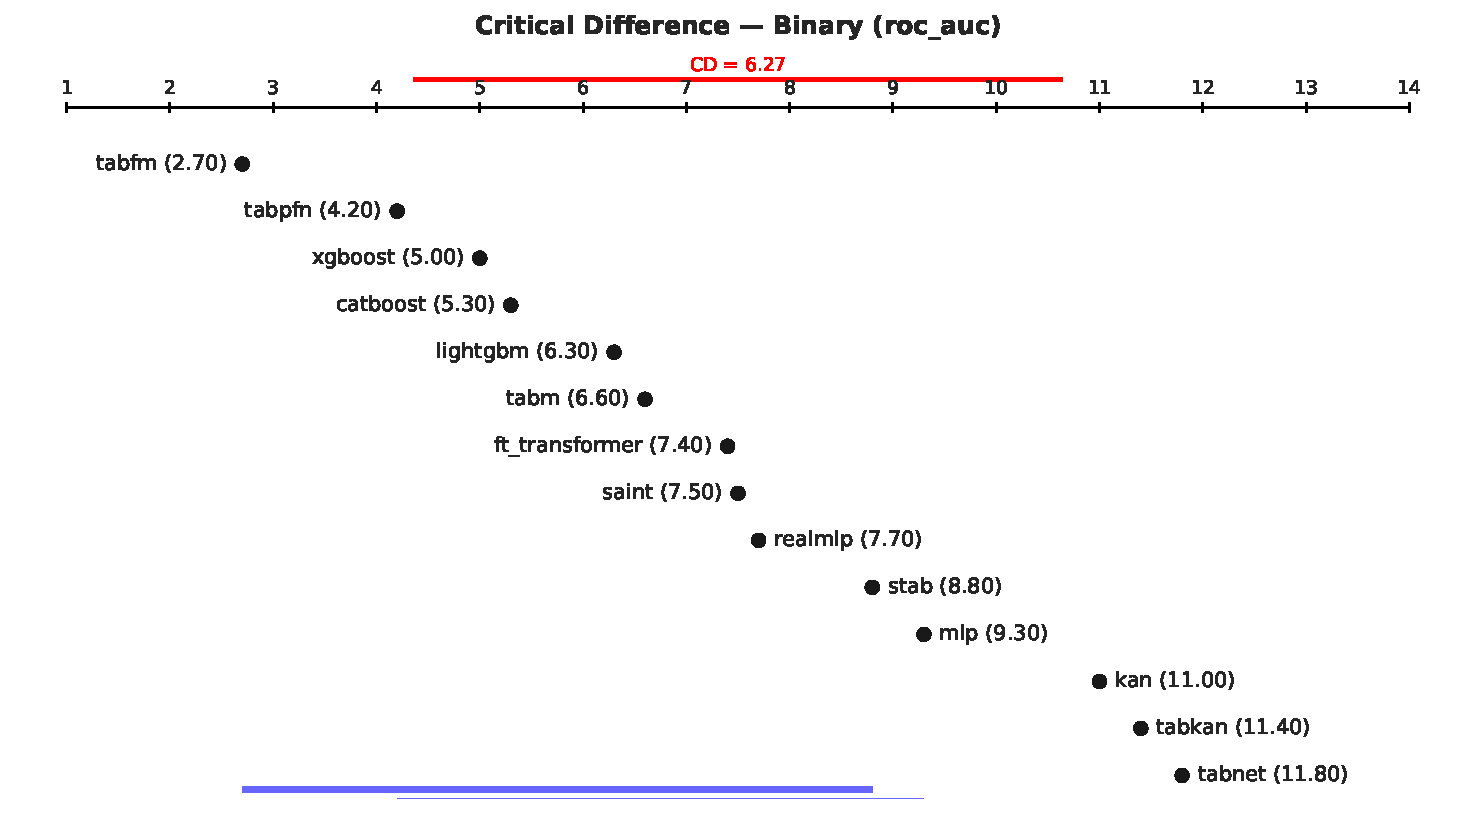
\includegraphics[width=0.85\linewidth]{figures/cd_diagram_binary.pdf}
\caption{Critical-distance (Nemenyi) diagram --- binary classification.
The leading pack is not separable by the post-hoc.}
\label{fig:cd}
\end{figure}

\subsection{Act II --- the cost axes}

Models that tie in accuracy differ radically in cost. Median training time
varies ${\sim}300\times$ (LightGBM/XGBoost ${\sim}0.7$~s; SAINT/STab
${\sim}200$~s); inference latency spans five orders of magnitude. Measured
on \texttt{adult}: XGBoost 0.33~\us/row; the fast tier includes the three
GBDTs and the MLP-like DL models (CatBoost 1.4; RealMLP 1.5; TabKAN 2.3;
MLP 2.4; KAN 3.1; TabM 3.5); attention costs tens of \us{} (TabNet 17;
FT-Transformer 29; SAINT 45); and the extreme belongs to the
heavy-inference paradigms --- TabPFN 7,416, STab 8,645 and TabFM
43,262~\us/row. The binary cost$\times$performance Pareto frontier is
\{TabPFN, XGBoost, LightGBM\}: all classical deep learning is dominated
(Fig.~\ref{fig:pareto}).
% results/latency/latency_adult.csv; notebooks/05_efficiency.ipynb

\begin{figure}[t]
\centering
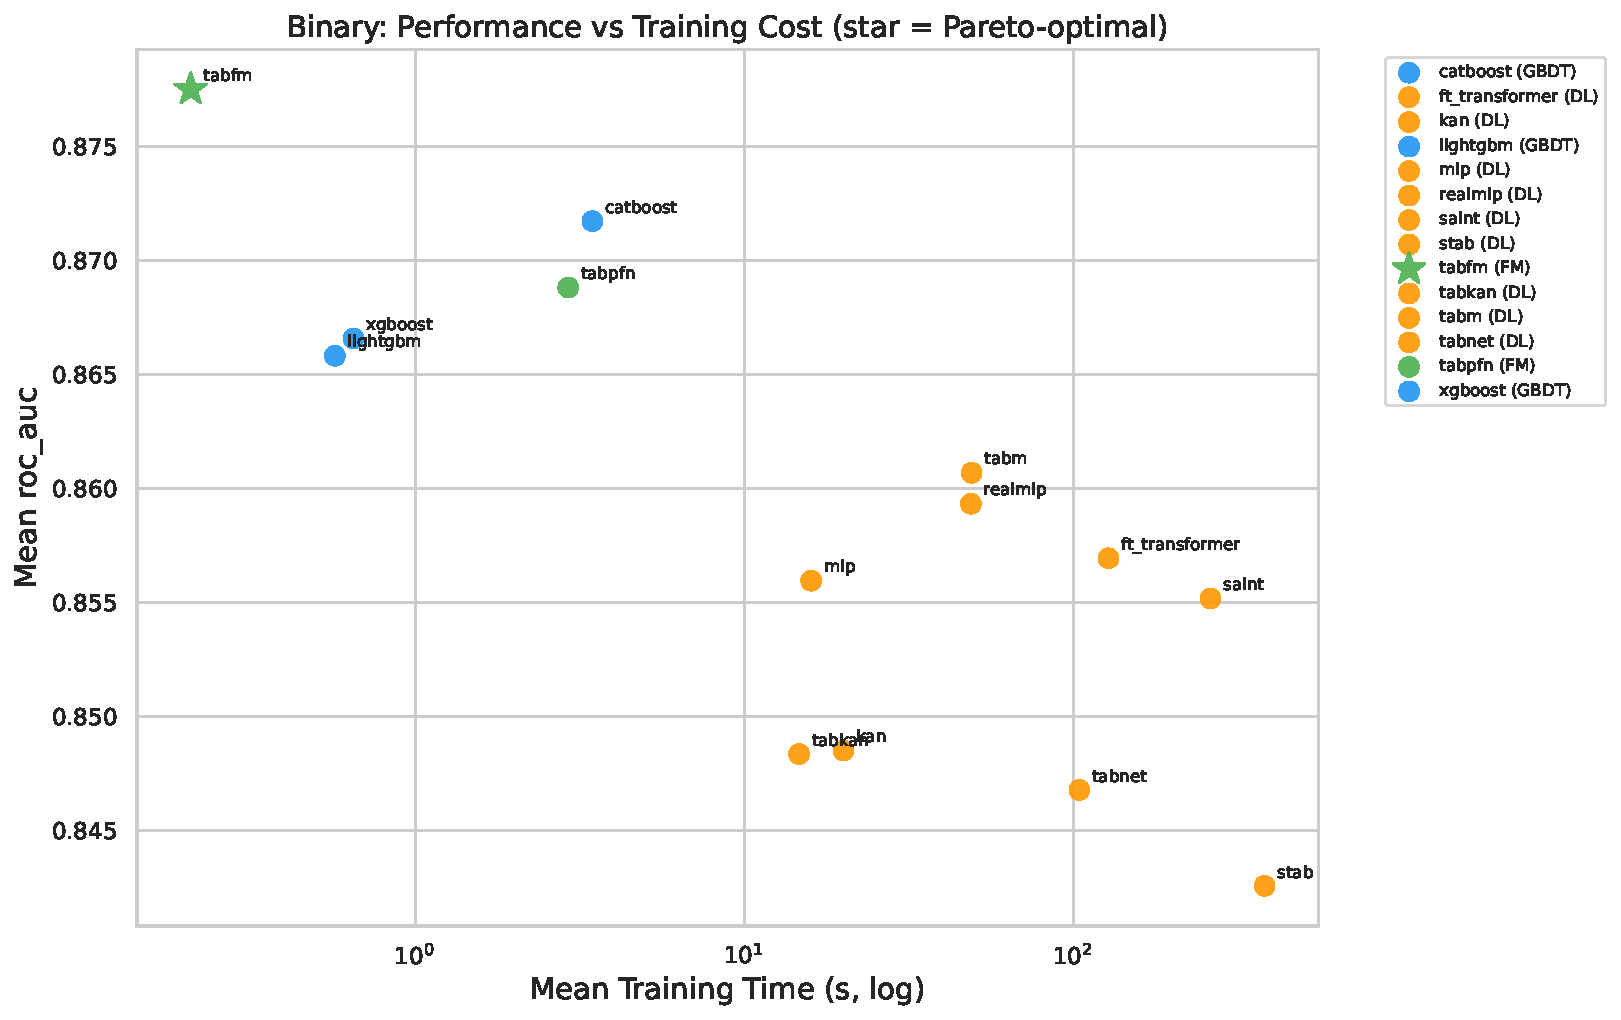
\includegraphics[width=0.9\linewidth]{figures/pareto_binary.pdf}
\caption{Performance $\times$ cost Pareto frontier (binary). Classical DL
is dominated by \{TabPFN, XGBoost, LightGBM\}.}
\label{fig:pareto}
\end{figure}

\subsection{Act III --- conditional reversals and the size axis}

The best family depends on problem structure: in multiclass ($N{=}3$,
descriptive) the 2024 DL generation takes the classical top; under severe
imbalance GBDTs gain relative advantage; at the categorical extreme
one-hot encoding penalizes attention; and TabPFN combines the best mean
rank with the best worst-case. Learning curves (6 models $\times$ 5
datasets $\times$ 3 seeds, from 500 samples to the full pool;
Fig.~\ref{fig:curves}) give the size axis its shape: the
GBDT$\leftrightarrow$DL leadership crossover is real and
dataset-specific --- on 3 of 5, DL overtakes and does not give the lead
back; on \texttt{adult}, the GBDT retakes it at $n \approx 4{,}000$ ---
and TabPFN is the best model on \emph{every} dataset in the
$n \leq 4{,}000$ regime, quantifying the few-shot niche of the zero-shot
paradigm.
% notebooks/10_learning_curves.ipynb

\begin{figure}[t]
\centering
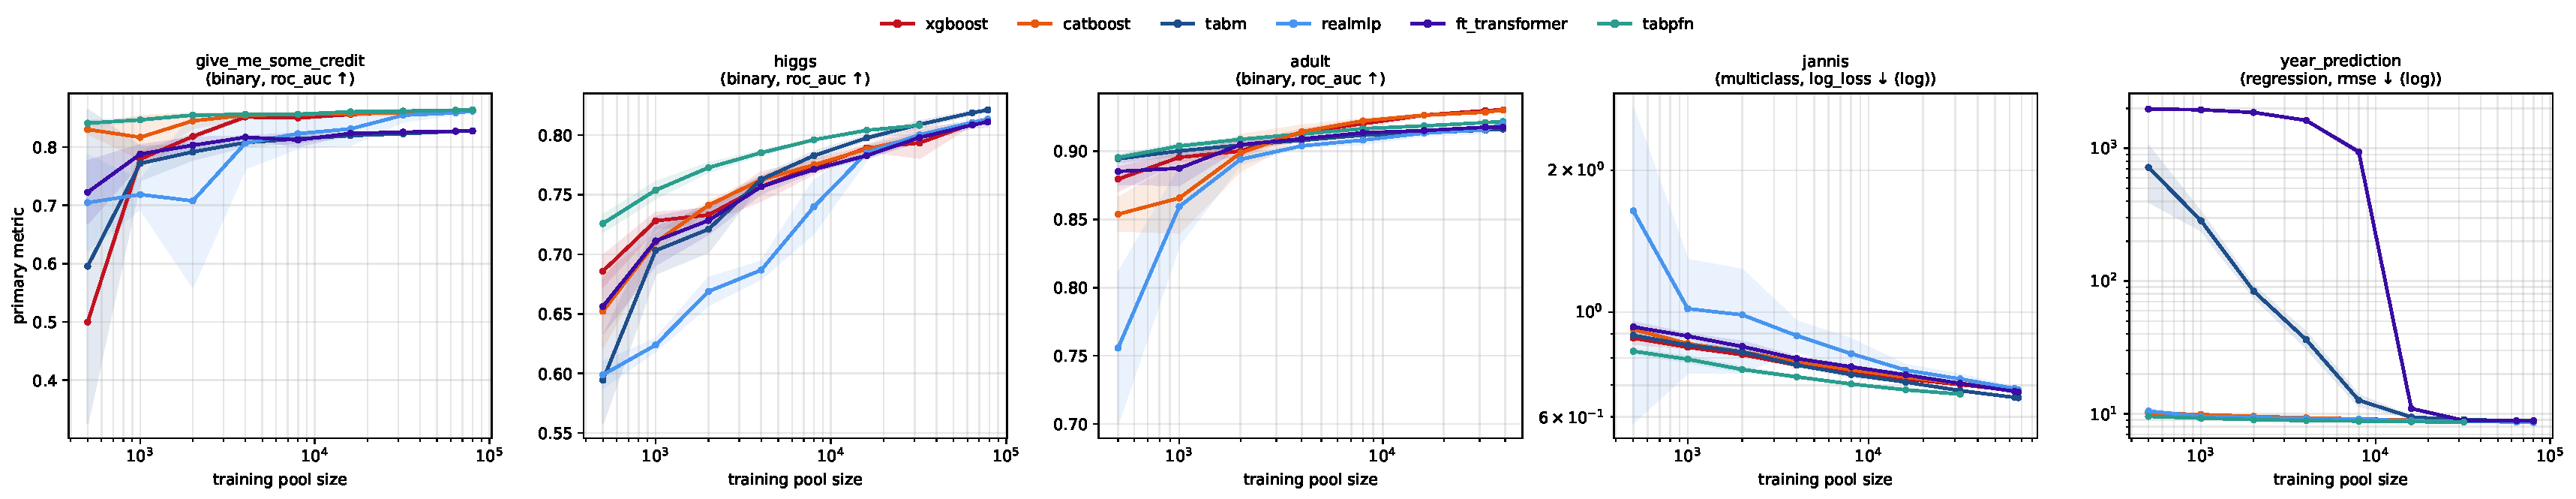
\includegraphics[width=\linewidth]{figures/learning_curves.pdf}
\caption{Learning curves (6 models $\times$ 5 datasets $\times$ 3 seeds).
The GBDT$\leftrightarrow$DL crossover is dataset-specific; TabPFN
dominates the $n \leq 4$k regime.}
\label{fig:curves}
\end{figure}

\subsection{Act IV --- the break of the tie (2026 generation)}

Expanding to 14 models reorganizes the narrative (Table~\ref{tab:ranks},
Fig.~\ref{fig:ranks}). TabFM leads the mean rank on all three tasks ---
2.7 binary, 1.0 (perfect) multiclass, 1.2 regression --- and is the single
best model on \textbf{13 of 18 datasets}, participating in 17. The Act~I
tie is correctly re-scoped as a portrait of the previous generation: it
was not tuned DL that caught up with GBDTs; it was pre-training that
overtook both. The statistical caution remains stated: with $k{=}14$ and
$N{=}10$, the Nemenyi CD is wide --- TabFM's separation rests on
cross-dataset consistency and on the Bayesian instrument, not on the
post-hoc.

\begin{table}[t]
\centering
\caption{Mean rank per task --- 2026 generation vs.\ reference ($k{=}14$
models; binary $N{=}10$, multiclass $N{=}3$, regression $N{=}5$).
Source: \texttt{notebooks/TABELA\_RESULTADOS.md}.}
\label{tab:ranks}
\begin{tabular}{lccc}
\toprule
 & Binary & Multiclass & Regression \\
\midrule
\textbf{TabFM}     & \textbf{2.7} & \textbf{1.00} & \textbf{1.2} \\
TabPFN             & 4.2          & 2.50          & 3.0 \\
Best classical     & XGBoost 5.0  & STab/TabM 3.67 & XGBoost 5.0 \\
KAN                & 11.0         & 12.0          & 9.8 \\
TabKAN             & 11.4         & 13.3          & 11.8 \\
\bottomrule
\end{tabular}
\end{table}

\begin{figure}[t]
\centering
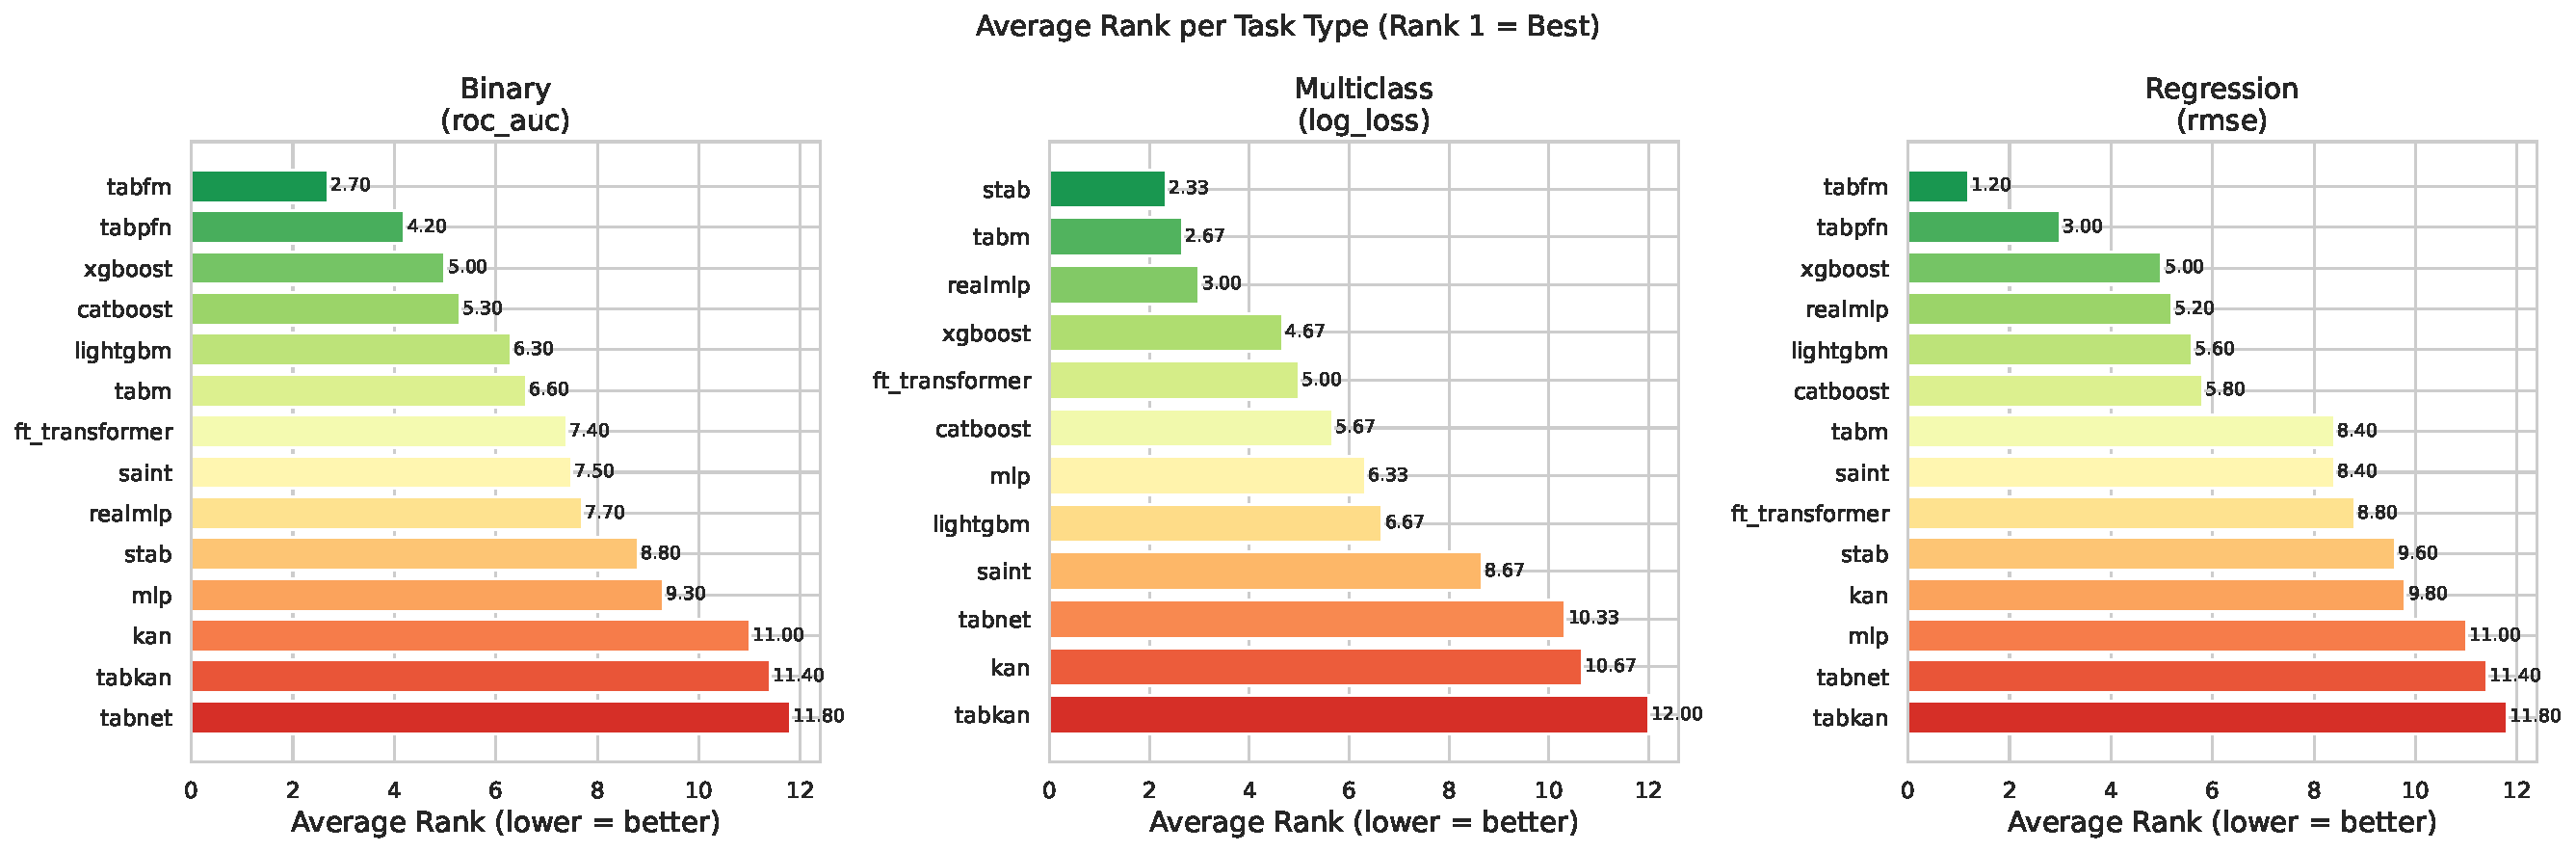
\includegraphics[width=0.9\linewidth]{figures/average_ranks.pdf}
\caption{Mean ranks of the 14 models. The 2026 generation (TabFM)
separates from the pack; the KANs occupy the bottom third.}
\label{fig:ranks}
\end{figure}

The counterweight is brutal, and it is the program's anchor finding: the
accuracy leader is the worst model in latency (43,262~\us/row under the
standard protocol --- $131{,}097\times$ XGBoost --- and more at larger
contexts, up to ${\sim}394$~ms/row on the largest regression dataset). The
decision question has changed from ``which family?'' to ``\emph{does the
foundation model's latency fit the use case?}''.

In the same movement, the independent test of the KANs produces the
valuable negative result: KAN (11.0/12.0/9.8) and TabKAN (11.4/13.3/11.8)
occupy the bottom third on all three tasks, with TabKAN behind even TabNet
in multiclass and regression --- under a uniform protocol, the original
paper's claims \citep{tabkan2025} do not hold (the likely explanation is
an under-tuned baseline), confirming the skeptical literature
\citep{kancritical2024}. As far as our dated verification reaches, this is
the family's first neutral test in a multi-criteria tabular benchmark. The
engineering counterpart deserves record: both live in the fast latency
tier (2--3~\us/row) --- the problem is performance, not cost.

\section{The validated decision framework}

\subsection{Negative result: meta-feature routing does not generalize}

The meta-learning literature suggests predicting the winning algorithm
from dataset meta-features. We test this with leave-one-dataset-out (LODO)
validation: a depth-2 tree trained on the remaining 17 datasets predicts
the winning family of the held-out one. Result: \textbf{hit rate 0.11
against a 0.44 majority-class baseline}. With $N{=}18$, learning the
routing is statistically infeasible --- and stating this under an explicit
protocol shields the framework from the overclaiming critique that
reaches part of the algorithm-recommendation literature. The tree remains
in the work as a descriptive illustration, never as a predictor.
% scripts/lodo_validation.py; results/aggregated/lodo_validation{,_14}.csv

\subsection{Positive result: the ``FM first'' policy}

As the alternative, we evaluate fixed policies by normalized regret (0 =
the recommended family contains the dataset's best model; 1 = it contains
only the worst):

\begin{table}[h]
\centering
\caption{Normalized regret of fixed policies under LODO.
Source: \texttt{results/aggregated/lodo\_validation\{,\_14\}.csv}.}
\label{tab:regret}
\small
\begin{tabular}{lcccc}
\toprule
Policy & mean @11 & median @11 & mean @14 & median @14 \\
\midrule
Tree (LODO)       & 0.228 & 0.145 & 0.051 & 0.000 \\
Always-GBDT       & 0.249 & 0.168 & 0.305 & 0.291 \\
Always-DL         & 0.189 & 0.132 & 0.313 & 0.349 \\
\textbf{Always-FM} & \textbf{0.115} & \textbf{0.018} & \textbf{0.021} &
\textbf{0.000} \\
\bottomrule
\end{tabular}
\end{table}

Already in the $\leq$2025 generation, ``use the foundation model by
default'' was the best fixed policy. With the 2026 generation, its median
regret drops to \textbf{zero}: in half or more of the datasets, the FM
family contains the best model. The question ``which family wins?''
dissolves --- and with it the value of any performance router.

\subsection{The resulting framework: decision by constraints}

What remains --- and what the framework's flowchart always encoded --- is
decision by constraints verifiable a priori: (1) \textbf{serving
latency/cost} --- if the budget is microseconds, the FM family is excluded
in native form (recovering it by distillation is the object of our second
activity, AI-2); (2) \textbf{architectural limits} ($>$10 classes, context
limit); (3) \textbf{intrinsic interpretability required} $\to$ GBDTs; (4)
\textbf{no active constraint} $\to$ foundation model, with TabPFN as the
mature option and TabFM as the frontier. The regret validation confirms
that these four questions capture the essential: the constraints are the
decision's real informative content.

\section{Limitations}

Small $N$ limits per-task power (regression $N{=}5$: Wilcoxon floor at
0.0625; multiclass $N{=}3$: descriptive); the \texttt{helena} dataset is
excluded twice by architectural limit; TabFM is evaluated at the pinned
v1.0.1 release, weeks old and without a peer-reviewed paper --- the
results are about that version and this is declared; LODO regret is
computed on the primary metric, not on preference-weighted multi-criteria
combinations; the model frontier changes on a cadence of months --- the
framework is dated by construction and versioned with the benchmark that
supports it.

\section{Conclusion}

The rule ``boosting always wins'' is not false --- it expired. It held as
a portrait of the generation up to 2025, where the top ties and 80\% of
variance is intra-family; in 2026, pre-training broke the accuracy tie and
inverted the cost axis: the best model in accuracy is the worst in
latency, by 4--5 orders of magnitude. The multi-criteria framework leaves
the LODO validation with a clearer role --- not predicting the winner
(infeasible), but encoding the constraints that actually decide --- and
the policy ``FM first, deviate on constraints'' has median regret zero.
The only obstacle to the optimal policy is serving cost; removing it by
distillation is the object of the companion activity (AI-2). Code,
configurations, seeds, per-experiment artifacts, and the public
corrections recorded along the study are in the repository
(\url{https://github.com/Gvascons/master-thesis}).

\bibliographystyle{abbrvnat}
\bibliography{refs}

\end{document}
